%versi 3 (22-07-2020)
\setcounter{secnumdepth}{4}
\chapter{Landasan Teori}
\label{chap:teori}

Pada bab ini akan menjelaskan dasar-dasar teori mengenai Ionic, berikut dengan cara untuk melakukan migrasi dari Ionic 3 ke Ionic 5. Akan dibahas pula aplikasi WSDC 2017 Bali saat ini. Cordova, dan Angular.

\section{WSDC 2017 Bali}
\label{sec:wsdc2017bali}

Aplikasi WSDC 2017 Bali digunakan untuk menunjang keberlangsungan acara WSDC 2017 yang diselenggarakan di Bali, Indonesia (Gambar \ref{fig:wsdcapp}). Aplikasi WSDC 2017 Bali dapat diunduh untuk sistem operasi {\it android} melalui URL \url{https://play.google.com/store/apps/details?id=org.wsdc2017indonesia.app&hl=en&gl=US}. Aplikasi ini dibangun dan dikembangkan oleh PT DNArtworks Komunikasi Visual yang rilis di Play Store pada tanggal 30 Juli 2017, dengan versi terakhir adalah versi 1.1.2 yang rilis pada 1 Agustus 2017. Selain rilis pada perangkat {\it android}, aplikasi ini juga rilis untuk perangkat bergerak berbasis sistem operasi iOS. Namun saat ini aplikasi tersebut sudah diturunkan dari App Store pada perangkat berbasis sistem opearsi iOS. Untuk membuka dan memakai aplikasi WSDC 2017 Bali saat ini, pengguna tidak diperlukan {\it login} agar dapat mengakses seluruh fitur yang tersedia. Lalu, untuk kepentingan skripsi ini, peneliti memiliki akses ke dalam kode program aplikasi WSDC 2017 Bali.

\begin{figure}[H]
     \centering
     \begin{subfigure}[b]{0.3\textwidth}
        \centering
    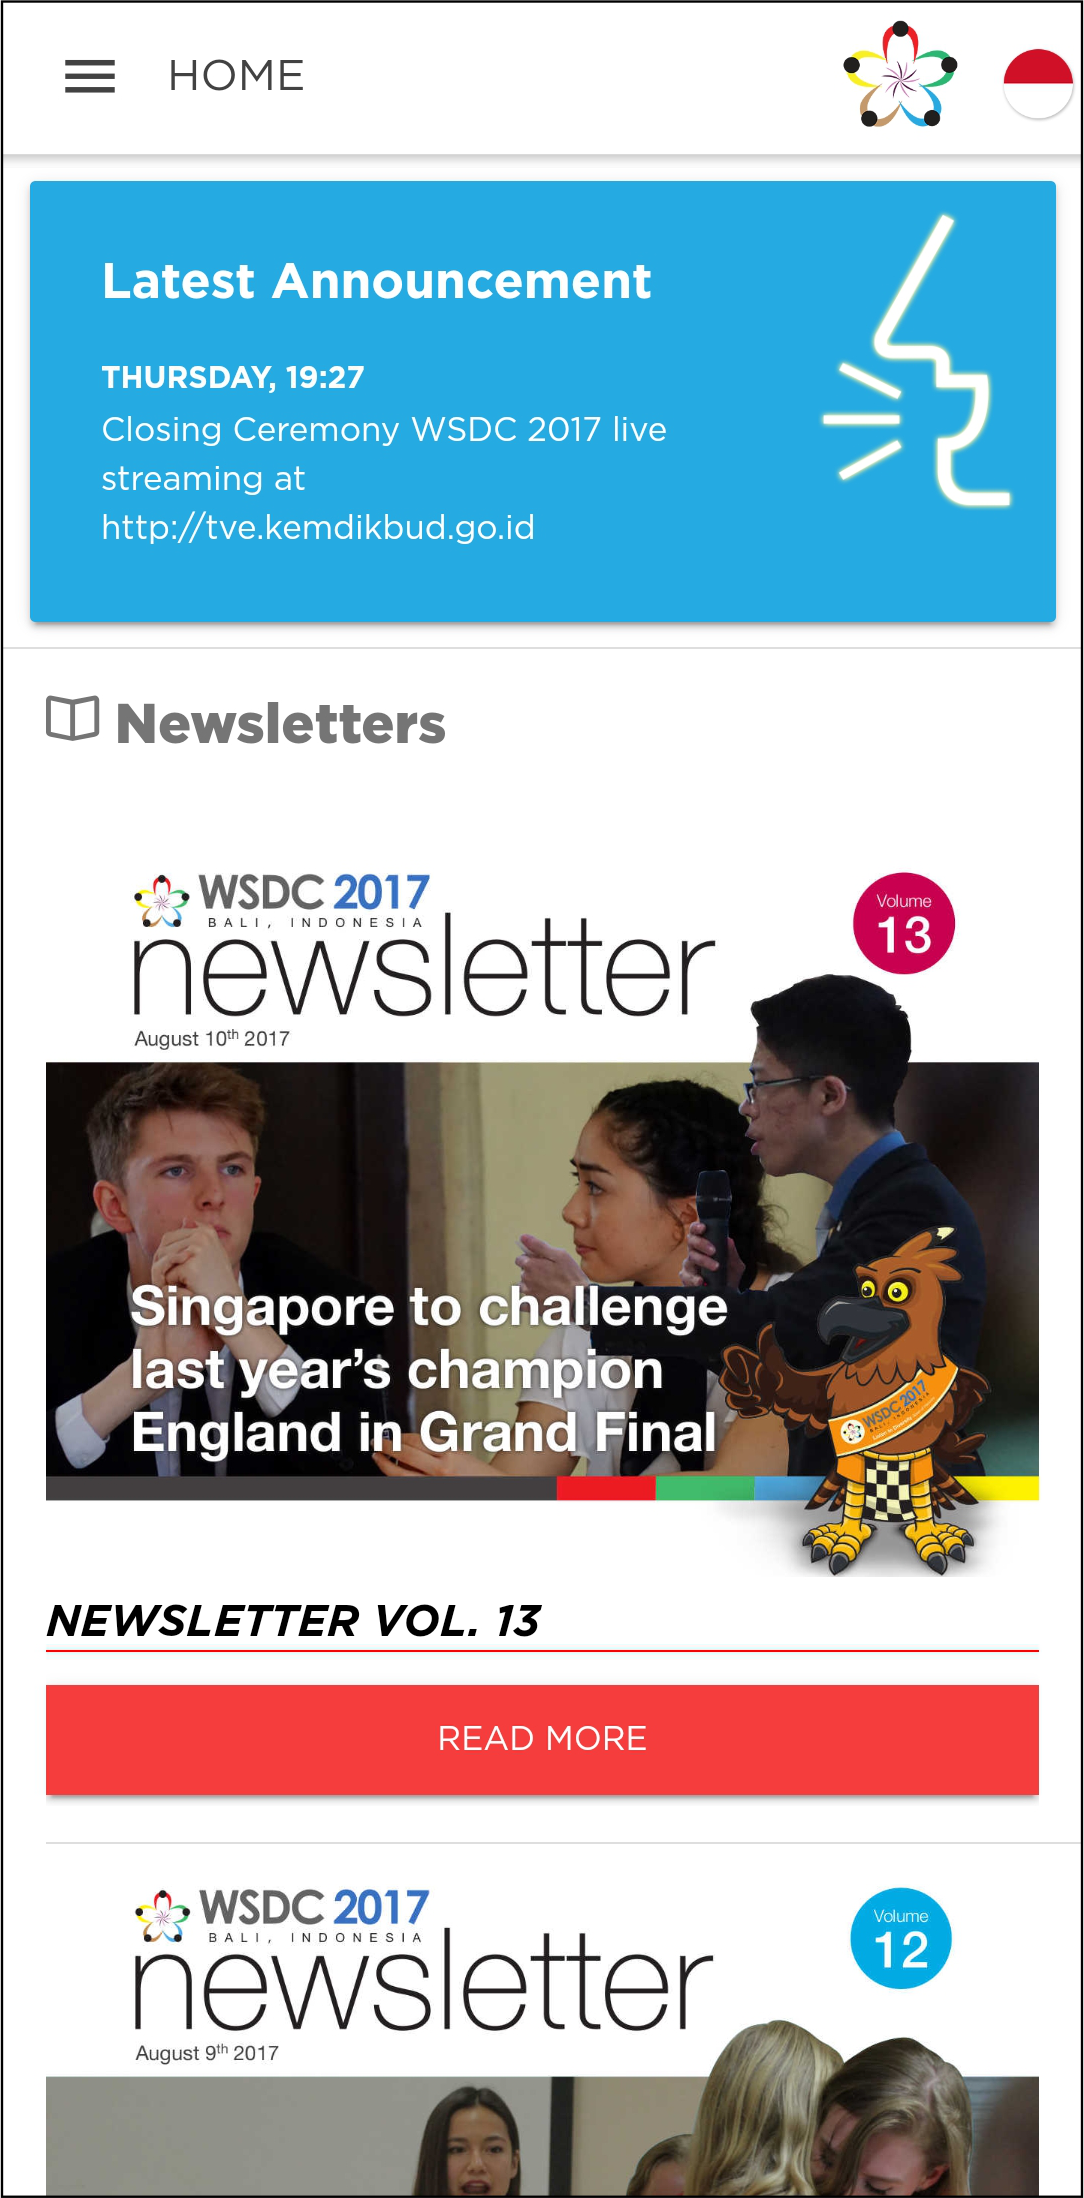
\includegraphics[scale=0.4]{Gambar/HomePage.png}
    \caption{Halaman Utama}
    \label{fig:wsdcapp}
     \end{subfigure}
     \hfill
     \begin{subfigure}[b]{0.3\textwidth}
    \centering
	    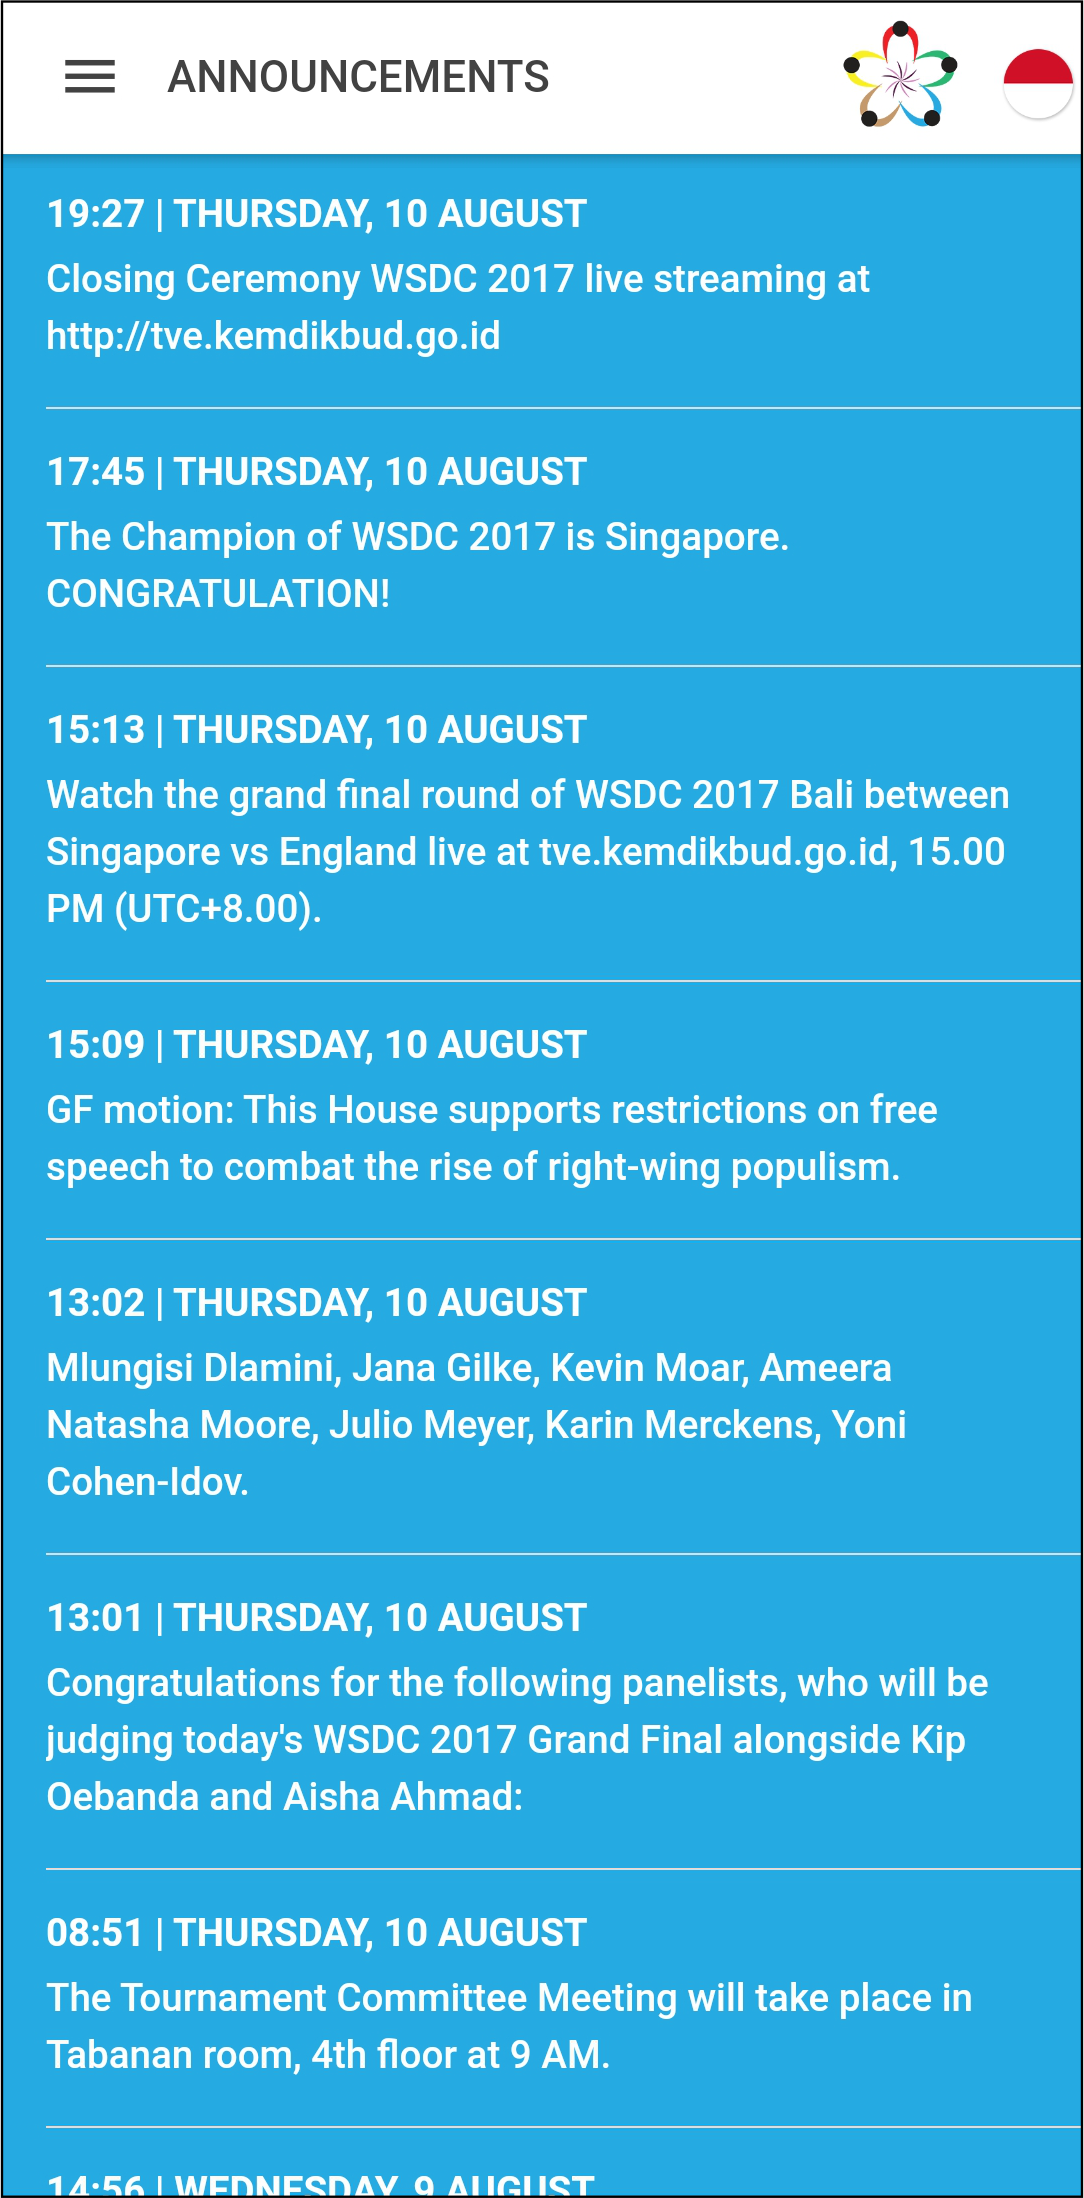
\includegraphics[scale=0.4]{Gambar/AnnouncementsPage.png}
	    \caption{Halaman {\it Announcements}}
	    \label{fig:wsdcAppAnnouncements}
     \end{subfigure}
     \hfill
     \begin{subfigure}[b]{0.3\textwidth}
         \centering
	    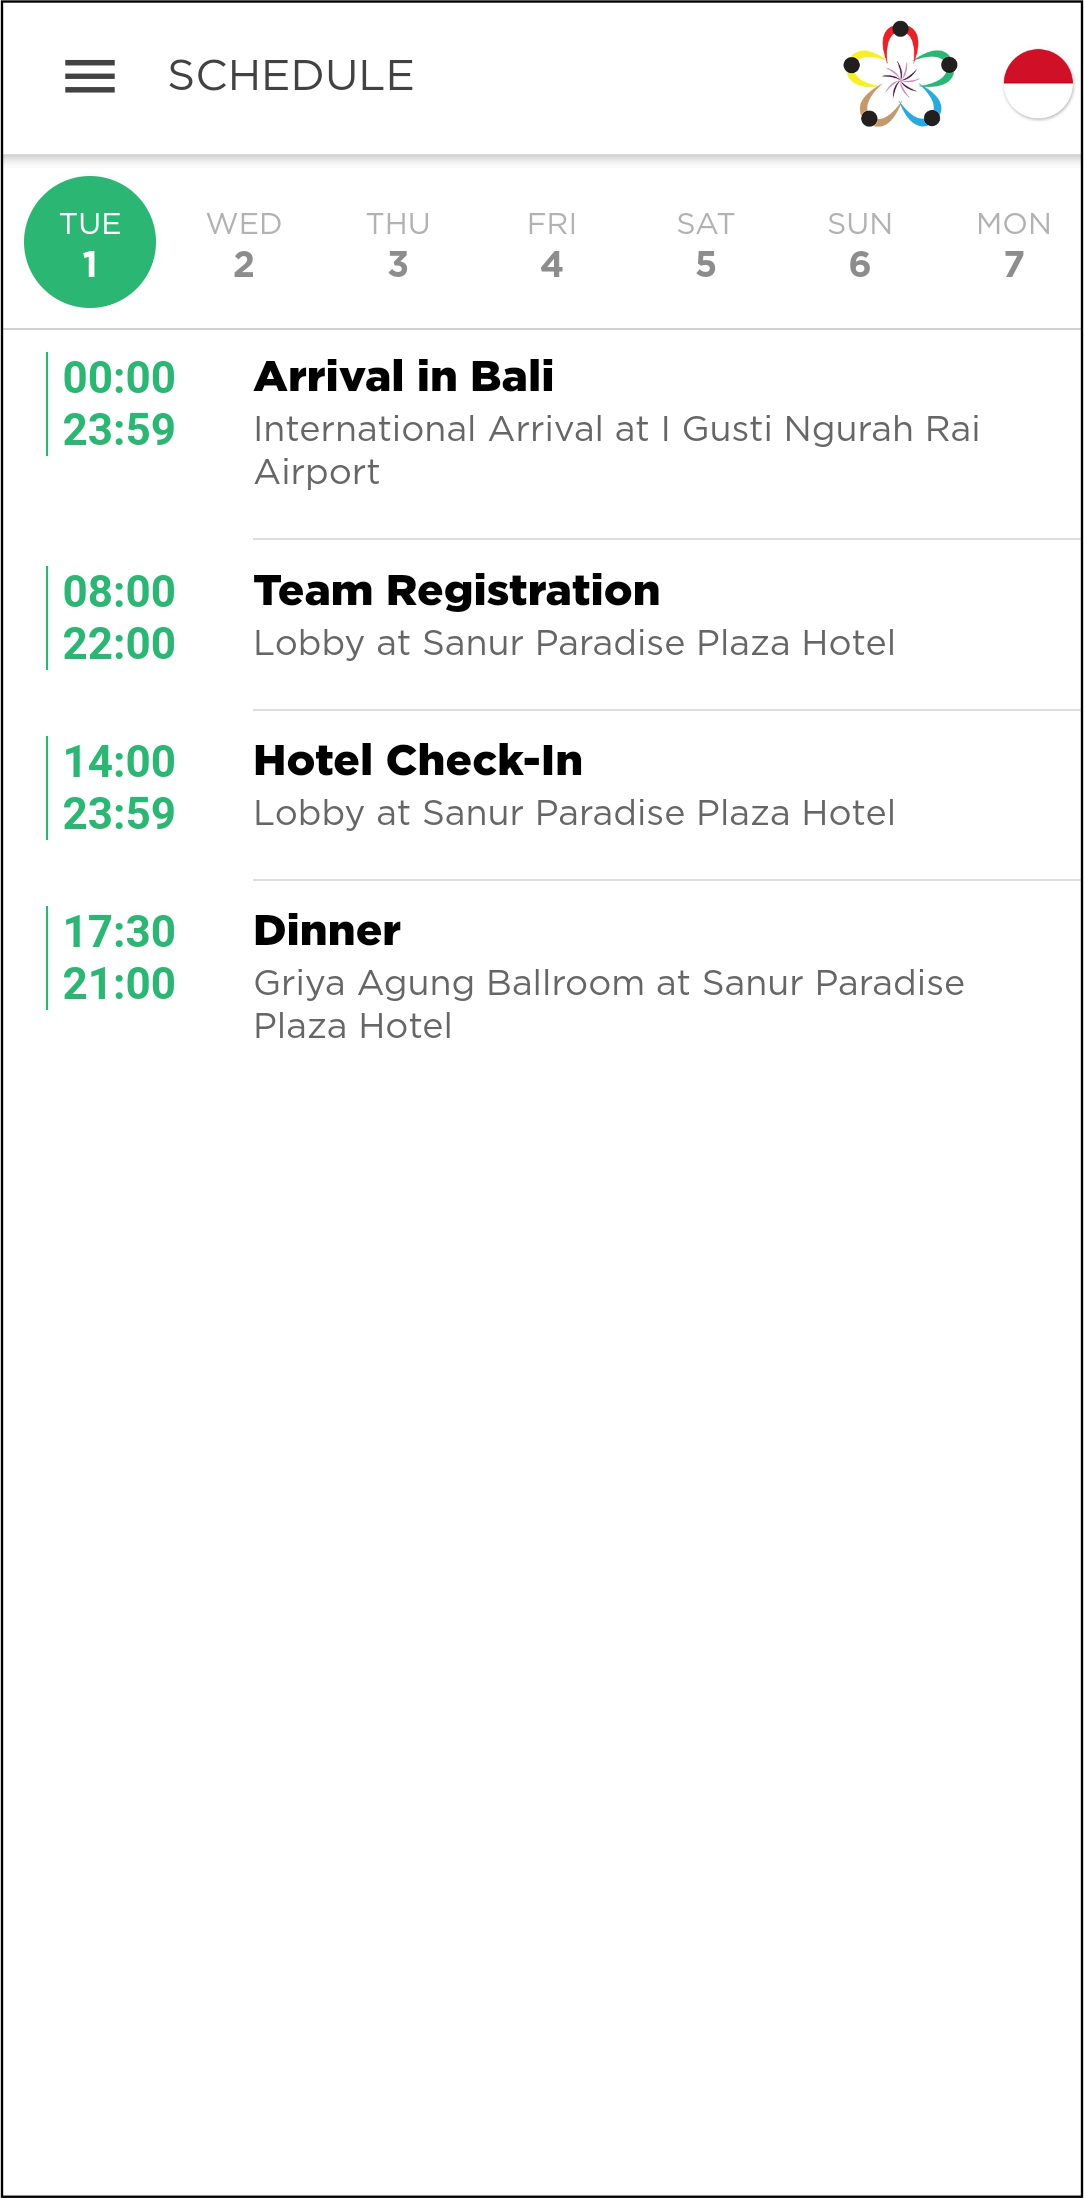
\includegraphics[scale=0.4]{Gambar/SchedulePage.png}
	    \caption{Halaman {\it Schedule}}
	    \label{fig:wsdcAppSchedule}
     \end{subfigure}
        \caption{Aplikasi WSDC 2017 Bali Saat Ini pada Perangkat Android}
        \label{fig:three graphs}
\end{figure}

Fitur-fitur yang terdapat di aplikasi WSDC 2017 Bali saat ini yaitu :

\begin{enumerate}
	\item {\it Announcements} : Pengguna dapat melihat pemberitahuan tentang berjalannya acara WSDC 2017 Bali (Gambar~\ref{fig:wsdcAppAnnouncements}).

	\item {\it Schedule} : Pengguna atau peserta WSDC 2017 Bali dapat melihat jadwal acara yang sudah diadakan (Gambar~\ref{fig:wsdcAppSchedule}).

	\item {\it Venues} : Pengguna atau peserta WSDC 2017 Bali dapat melihat berbagai macam lokasi acara, mulai dari lokasi upacara, lokasi kompetisi, dan lokasi wisata edukasi. Masing-masing dari lokasi tersebut dapat menunjukan arah dan jarak dari lokasi tempat pengguna berada (Gambar~\ref{fig:wsdcAppVenues}).

	\item Info : Pengguna dapat melihat informasi terkait dengan tim pengembang dari aplikasi WSDC 2017 Bali, kontak-kontak penting yang dapat dihubungi, dan kosa kata penting dalam Bahasa Indonesia (Gambar~\ref{fig:wsdcAppInfo}).

	\item {\it Draw} : Pengguna dapat melihat melihat pembagian {\it venue} dan kubu proposisi atau oposisi dari hasil pengundian untuk para negara peserta (Gambar~\ref{fig:wsdcAppDraw}).

	\item {\it Result} : Pengguna dapat melihat informasi terkait hasil dari pertandingan pada semi final, perempat final, dan perdelapan final (Gambar~\ref{fig:wsdcAppResult}).
\end{enumerate}

\begin{figure}[H]
     \centering
     \begin{subfigure}[b]{0.21\textwidth}
        \centering
	    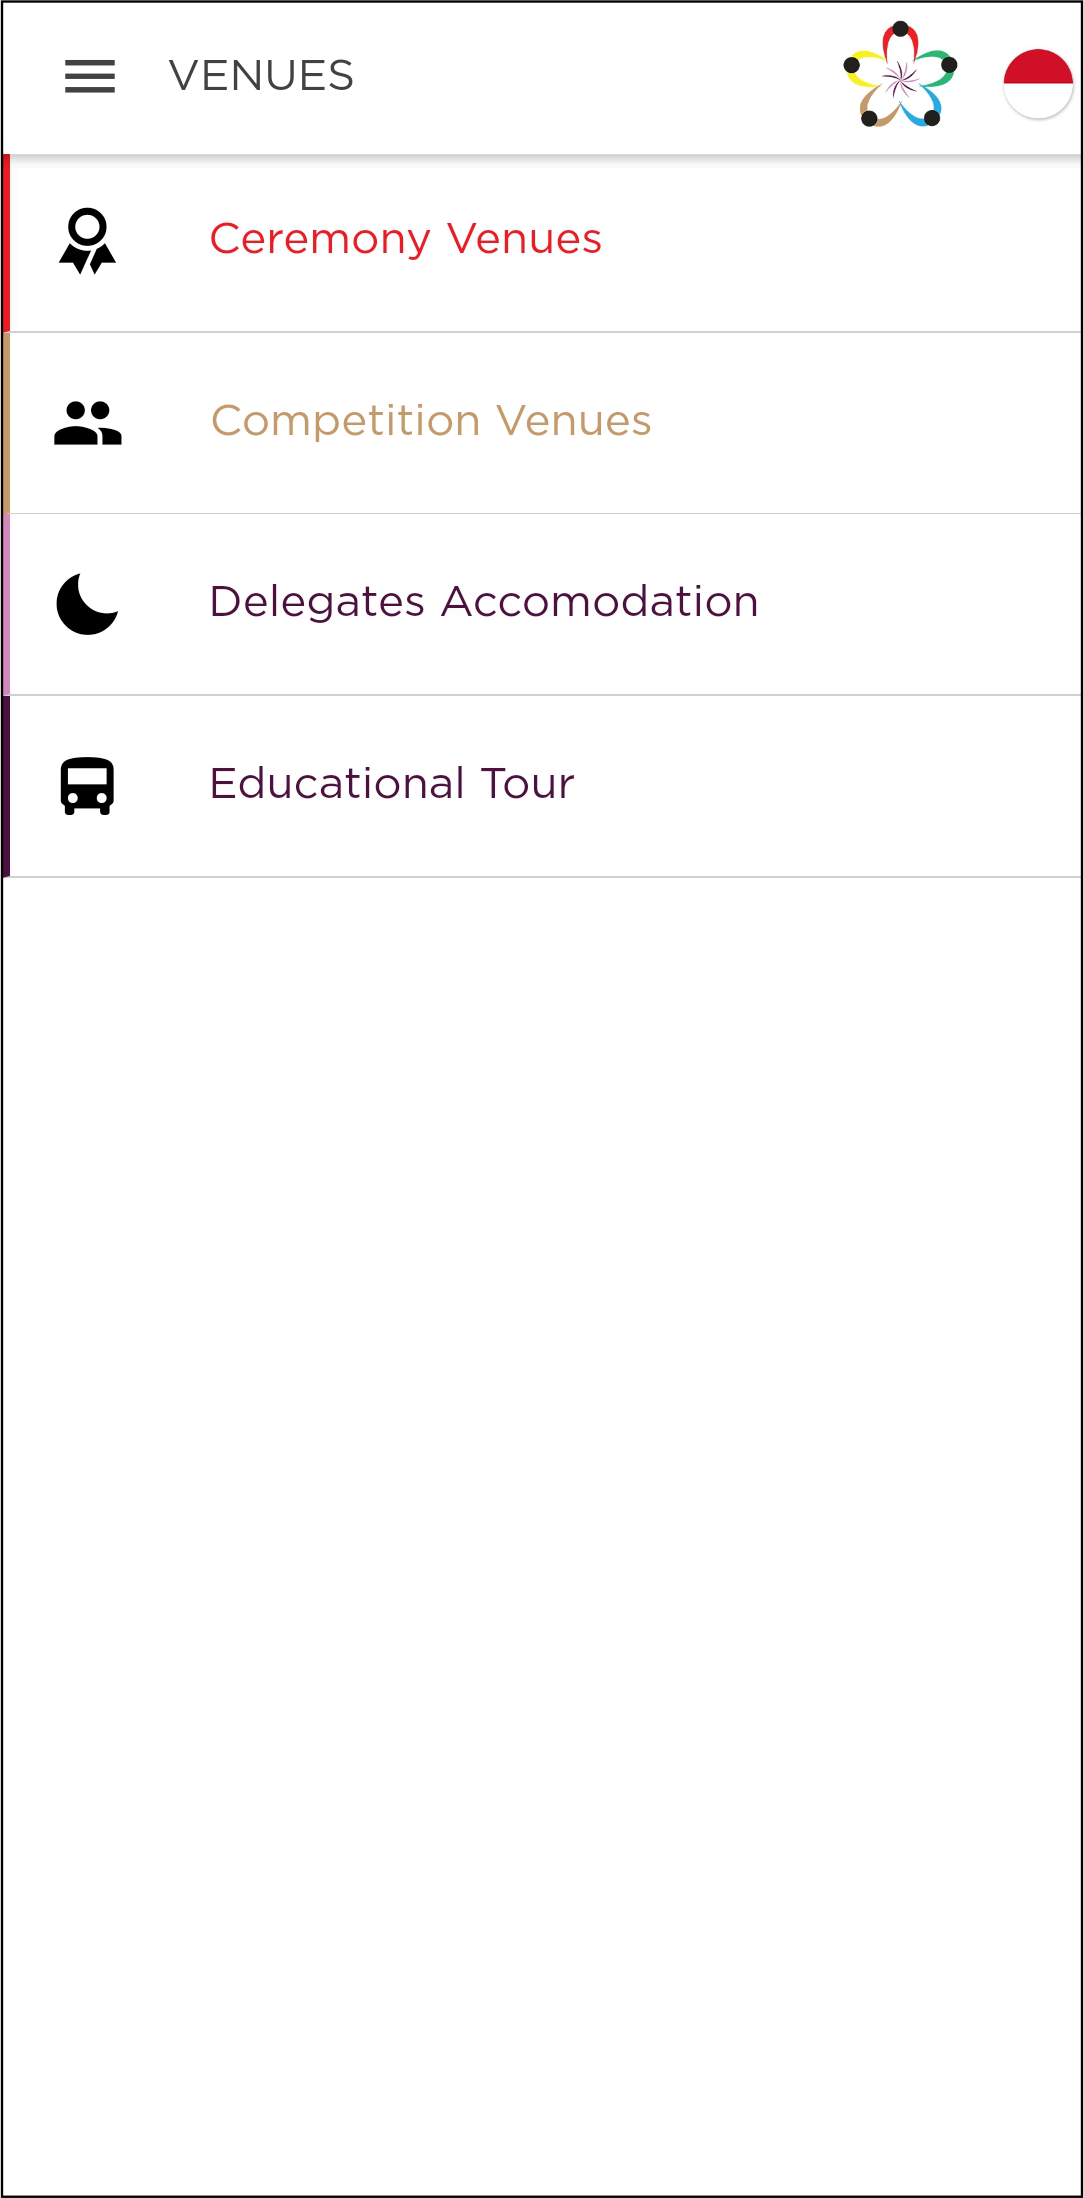
\includegraphics[scale=0.4]{Gambar/VenuePage.png}
	    \caption{Halaman {\it Venues}}
	    \label{fig:wsdcAppVenues}
     \end{subfigure}
     \hfill
     \begin{subfigure}[b]{0.247\textwidth}
    \centering
	    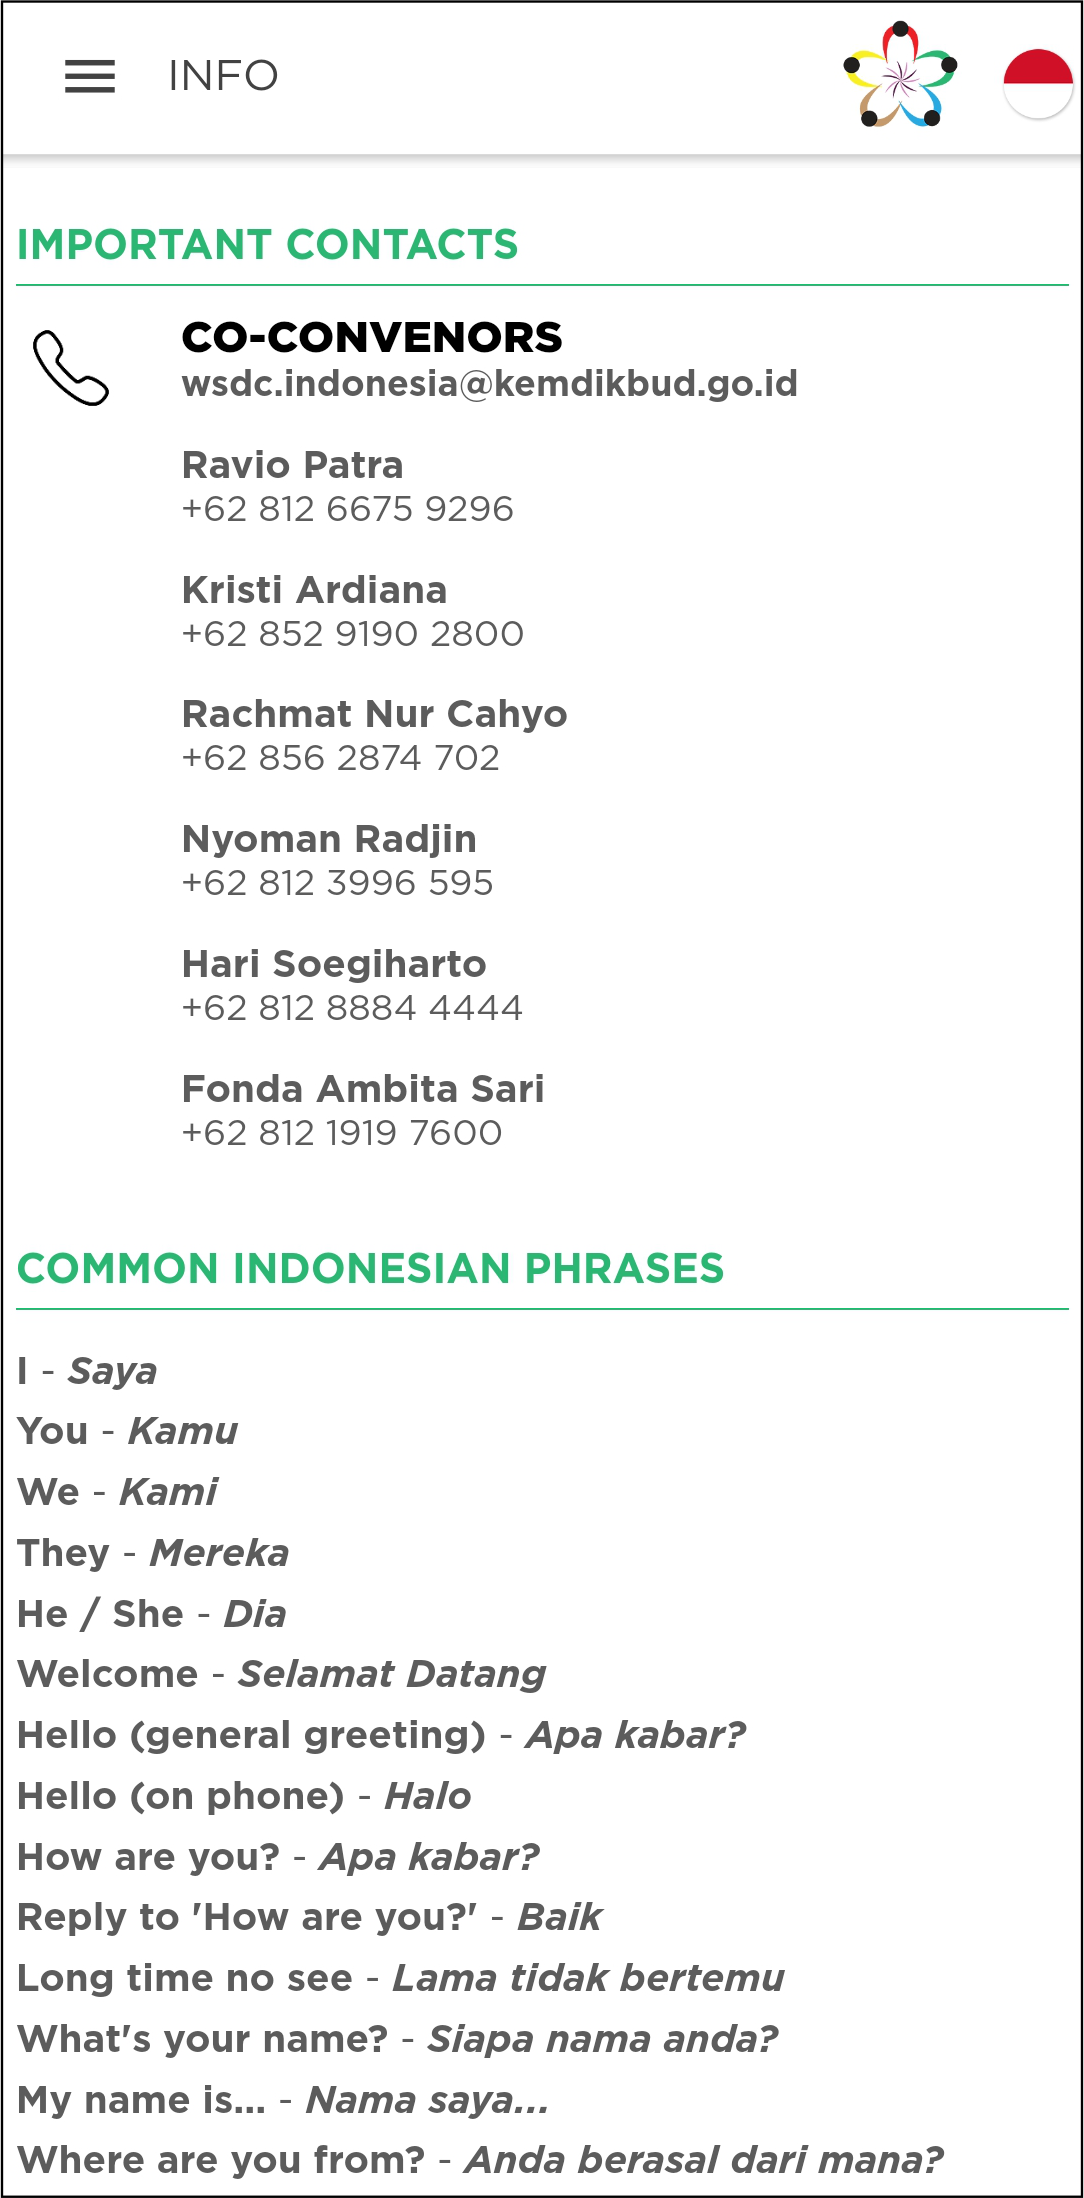
\includegraphics[scale=0.4]{Gambar/InfoPage.png}
	    \caption{Halaman Info}
	    \label{fig:wsdcAppInfo}
     \end{subfigure}
	\begin{subfigure}[b]{0.247\textwidth}
    \centering
	    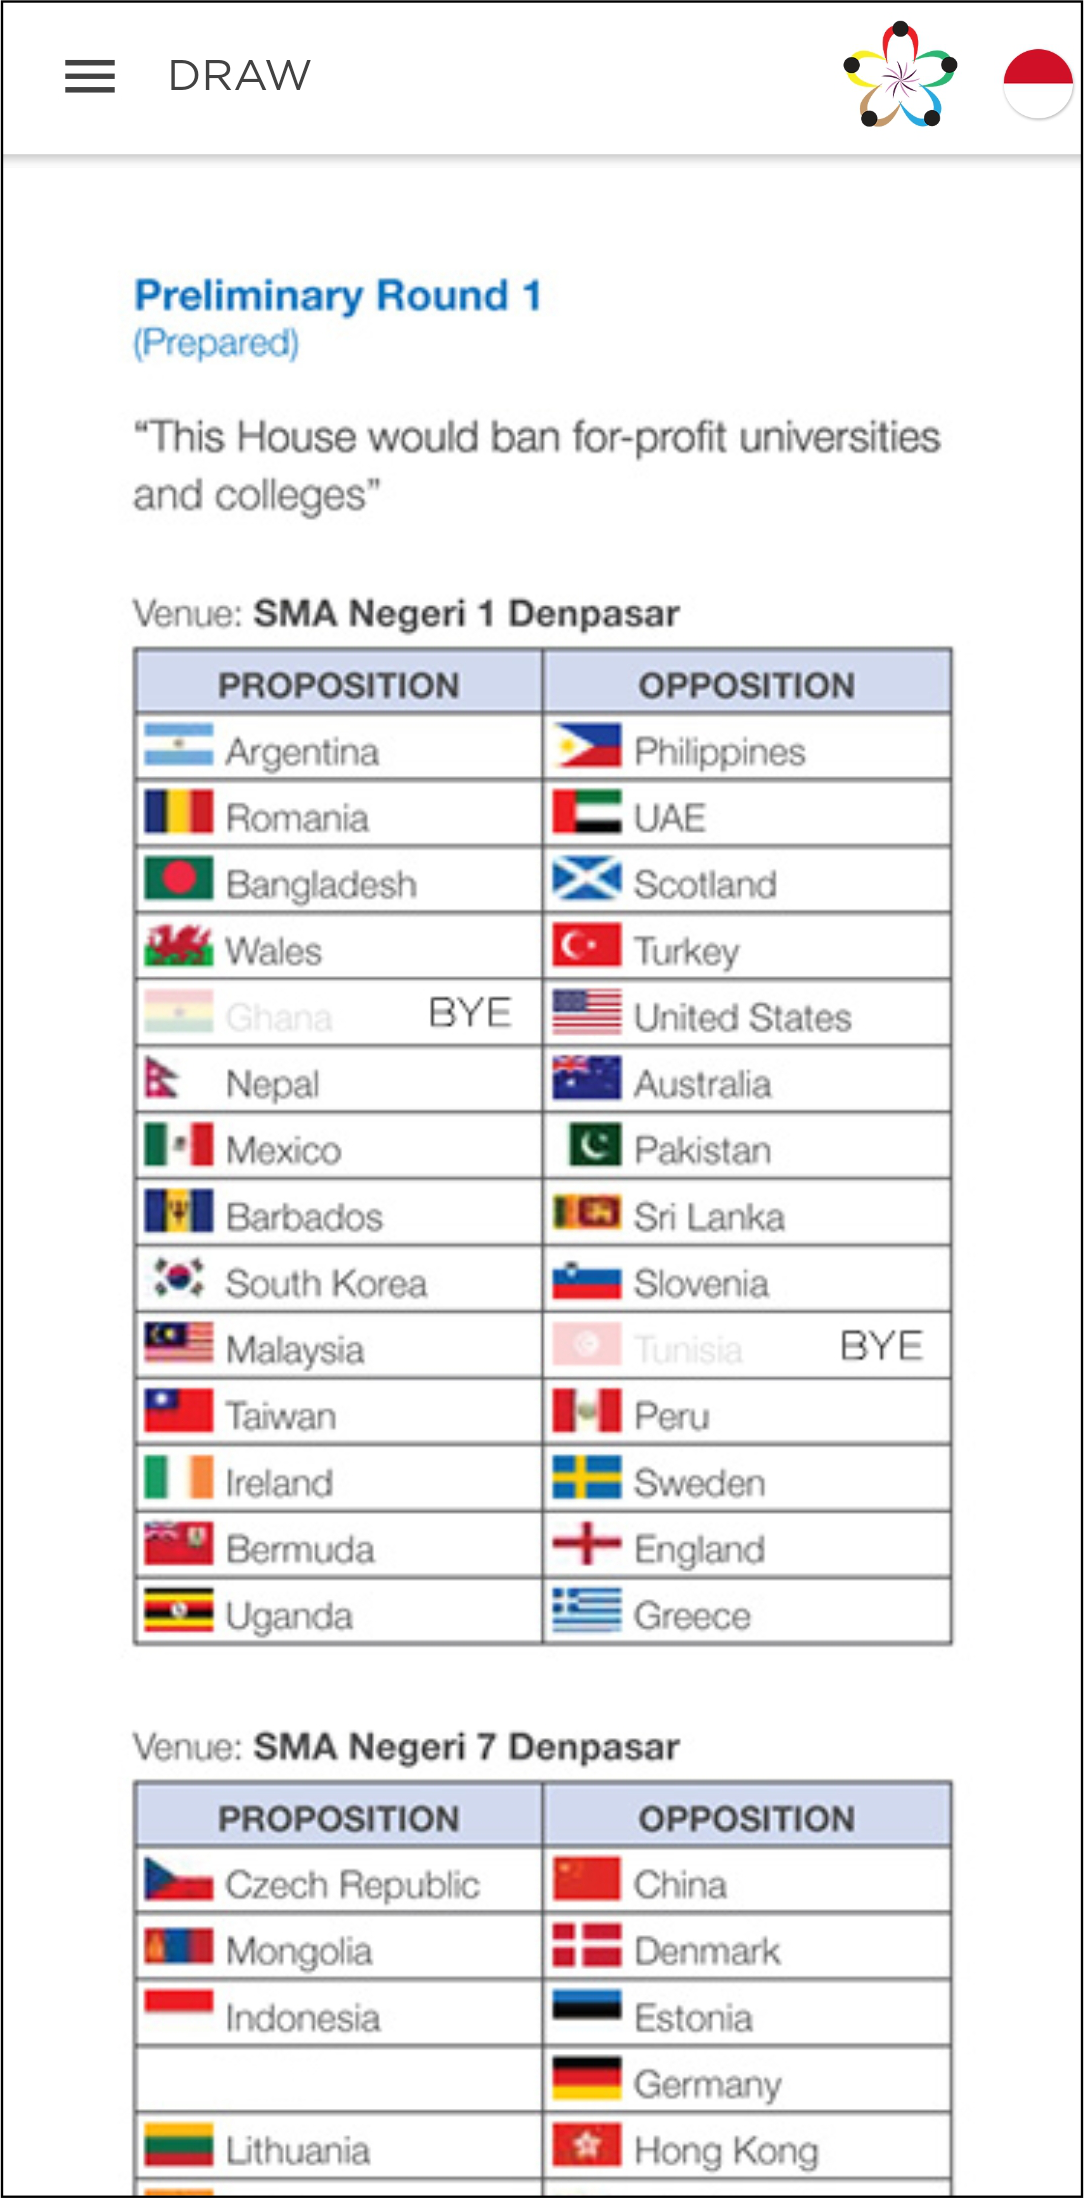
\includegraphics[scale=0.4]{Gambar/DrawPage.png}
	    \caption{Halaman {\it Draw}}
	    \label{fig:wsdcAppDraw}
     \end{subfigure}
	\begin{subfigure}[b]{0.247\textwidth}
    \centering
	    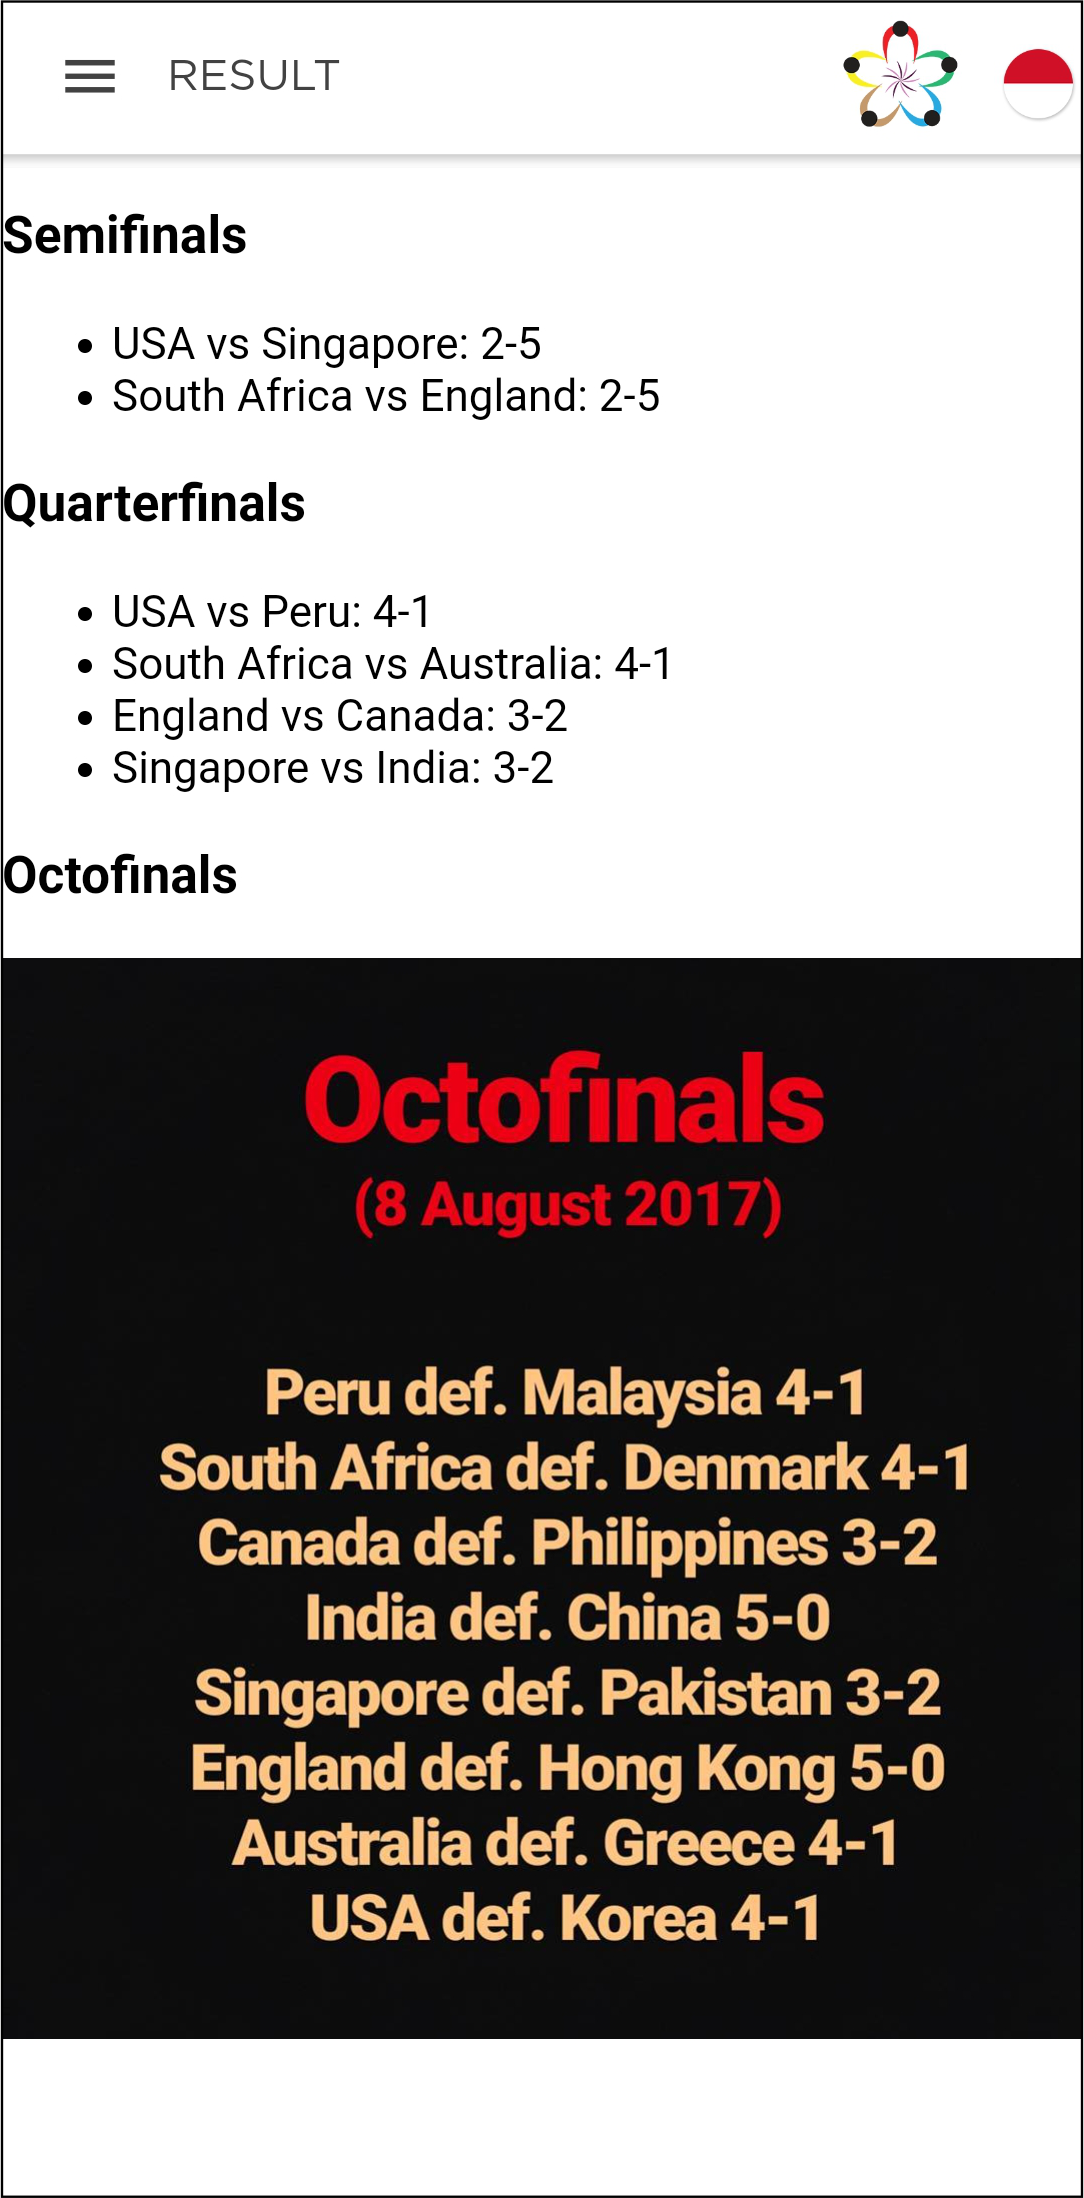
\includegraphics[scale=0.4]{Gambar/ResultPage.png}
	    \caption{Halaman {\it Result}}
	    \label{fig:wsdcAppResult}
     \end{subfigure}
	\caption{Aplikasi WSDC 2017 Bali Saat Ini pada Perangkat Android}
        \label{fig:three graphs}
\end{figure}



\section{Ionic {\it Framework}}
\label{sec:ionicframework} 
 
Ionic Framework merupakan sebuah kerangka kerja {\it open source} lintas platform yang memungkinkan untuk mengembangkan aplikasi hibrida yang bekerja pada berbagai macam platform seluler seperti {\it android}, iOS, dan Windows~\cite{waranashiwar:18:ionic}. Ionic memiliki berbagai macam \textit{front-end library} dan \textit{User Interface}(UI) {\it Components} yang digunakan untuk  perancangan aplikasi menggunakan teknologi web seperti HTML, CSS, dan Javascript, dengan integrasi untuk berbagai \textit{framework} seperti Angular, React, dan Vue. Saat pertama kali dibuat, Ionic menggunakan AngularJS. Namun, seiring saat Angular versi 2 yang menggunakan Typescript dirilis, Ionic versi 2 dan selanjutnya menggunakan Angular. Lalu, pada tahun 2019, Ionic mendukung penggunaan \textit{framework} lain selain Angular, yaitu React dan Vue. Di dalam Ionic, Angular digunakan untuk membangun aplikasi dan perutean, sehingga aplikasi dapat sejalan dengan ekosistem Angular lainnya. Ionic menyediakan {\it toolkit} Angular untuk membangun aplikasi dan terintegrasi dengan Angular CLI resmi yang menyediakan fitur khusus untuk aplikasi Ionic Angular. Pada saat skripsi ini dibuat, Ionic versi terbaru adalah Ionic versi 5, sedangkan Angular yang digunakan adalah Angular versi 12. 

\subsection{Native API}
\label{subsec:nativeApi}
Native API memungkinkan pengembangan aplikasi langsung terintegrasi ke dalam {\it platform}. Pengembang dapat membuat aplikasi pada perangkat {\it mobile} untuk dapat diimplementasikan ke berbagai {\it platform}, seperti IOS, dan Android, setelah pengembangan selesai di dalam {\it framework native} tanpa perlu perubahan, dan tidak mempengaruhi peforma dari aplikasi tersebut~\cite{griffith:17:mobile}. 

Ionic mendukung komunikasi dengan menggunakan Native API yang terintegrasi untuk menambahkan fungsionalitas ke dalam aplikasi Ionic apapun dengan menggunakan Capacitor atau Cordova. Dengan terpasangnya Ionic Native, maka aplikasi akan memiliki antar muka yang diperlukan untuk berinteraksi dengan salah satu plug-in, yaitu Capacitor atau Cordova.

\subsubsection{Capacitor}
\label{subsec:capacitor}
Penjelasan singkat mengenai capacitor di ionic

\subsubsection{Cordova}
\label{subsec:cordova}
Penjelasan lebih lengkap mengenai cordova, karena akan dipakai nantinya di aplikasi WSDC

\subsection{UI Component}
\label{subsec:uiComponent}
Penjelasan apa saja ui component yang ada pada Ionic
%2.2.1 Native API
%2.2.1.1 Capacitor
%2.2.1.2 Cordova
%2.2.2 UI Component 

\subsection{Migrasi Ionic 3 ke Ionic 5}
\label{subsec:migrasi}
%Aplikasi WSDC Bali 2017 saat ini menggunakan {\it framework} Ionic versi 3 yang sudah tidak didukung lagi. Maka dari itu dilakukan pembaruan aplikasi WSDC 2017 Bali ke dalam {\it framework} Ionic versi 5. 

Untuk melakukan migrasi dari Ionic 3 ke Ionic 5 memerlukan dua tahap, yaitu migrasi dari Ionic 3 ke Ionic 4, dan migrasi Ionic 4 ke Ionic 5. Tahapan migrasi tersebut adalah sebagai berikut:

%---START ENUM SECTION MIGRASI IONIC 3 KE IONIC 5---%
\begin{enumerate}
	\item Migrasi Ionic 3 ke Ionic 4 \\
	Ada beberapa langkah untuk melakukan migrasi dari Ionic 3 ke dalam Ionic 4, yaitu:
	

	%---START ENUM MIGRASI IONIC 3 KE IONIC 4---%
	\begin{enumerate}
		\item Membuat Projek Ionic Baru \\
		Untuk membuat projek Ionic baru tanpa {\it template} apapun dengan menggunakan perintah \textbf{ionic start myApp blank} dan memilih Angular sebagai {\it framework}nya.
		\begin{lstlisting}[language=php, caption=Perintah Membuat Projek Ionic Baru]
			ionic start myApp blank
		\end{lstlisting}
		
		\item Menyalin {\it Root-level Items} \\
		Menyalin seluruh {\it Root-level Items} pada Ionic versi 3 dengan direktori yang sama atau dengan beberapa perubahan. Terdapat beberapa perubahan baik itu nama maupun letak dari suatu fungsi atau berkas. Perubahan tersebut yaitu:

		%---START ITEMIZE MENYALIN ROOT LEVEL---%
		\begin{itemize}

			\item Angular
			%---START ITEMIZE ANGULAR---%
			\begin{itemize}
				\item HttpClient \\
				Pada Angular versi 4 keatas, objek {\it response} secara {\it default} merupakan JSON, jadi tidak perlu diubah kembali menjadi JSON.
			\end{itemize}
			%---END ITEMIZE ANGULAR---%


			\item {\it Imports} \\
			Terjadi perubahaan dalam mengimpor {\it package} di Ionic 3 dan Ionic 4. Daftar perubahan tersebut adalah sebagai berikut :
			%---START ITEMIZE IMPORT---%
			\begin{itemize}
				\item Angular HTTP \\
				Pada Ionic 3 : @angular/http\\
				Terdapat perubahan pada Ionic 4 menjadi : @angular/common/http
	
				\item Ionic Angular \\
				Pada Ionic 3 : ionic-angular  \\
				Terdapat perubahan pada Ionic 4 menjadi : @ionic/angular
	
				\item {\it In App Browser} \\
				Pada Ionic 3 : @ionic-native/in-app-browser \\
				Terdapat perubahan pada Ionic 4 menjadi : @ionic-native/in-app-browser/ngx
			\end{itemize}
			%---END ITEMIZE IMPORT---%
	

			\item Ionic {\it Component} \\
			Terjadi perubahaan pada Ionic {\it Component} di Ionic 3 dan Ionic 4. Daftar perubahan tersebut adalah sebagai berikut :
			%---START ITEMIZE COMPONENT---%
			\begin{itemize}
				\item {\it Button} \\
				Pada Ionic 3 : <button>  \\
				Terdapat perubahan pada Ionic 4 menjadi : <ion-button>
			\end{itemize}
			%---END ITEMIZE COMPONENT---%
	

			\item Perbedaan Direktori Berkas \\
			Terjadi perubahaan direktori pada berkas di Ionic 3 dan Ionic 4. Daftar perubahan tersebut adalah sebagai berikut :
			%---START ITEMIZE PERBEDAAN DIREKTORI BERKAS---%
			\begin{itemize}
				\item {\it Global Styling} \\
				Pada Ionic 3 : src/app/app.scss \\
				Terdapat perubahan pada Ionic 4 menjad : src/global.scss

				\item {\it Pages} \\
				Pada Ionic 3 : src/pages  \\
				Terdapat perubahan pada Ionic 4 menjad : src/app/pages
			\end{itemize}
			%---END ITEMIZE PERBEDAAN DIREKTORI BERKAS---%
	

			\item Penamaan Berkas \\
			Terjadi perubahaan penamaan pada berkas di Ionic 3 dan Ionic 4. Daftar perubahan tersebut adalah sebagai berikut:
			%---START ITEMIZE PENAMAAN BERKAS---%
			\begin{itemize}
				\item {\it Page} \\
				Contoh perbedaan nama {\it file} pada folder Pages adalah sebagai berikut :\\
				Pada Ionic 3 : home.html  \\
				Terdapat perubahan pada Ionic 4 menjad : home.page.html
	
				\item {\it App} \\
				Contoh perbedaan nama {\it file} pada direktori App adalah sebagai berikut : \\
				Pada Ionic 3 : app.html \\
				Terdapat perubahan pada Ionic 4 menjad : app-component.html
			\end{itemize}
			%---END ITEMIZE PENAMAAN BERKAS---%


			\item {\it Routing}
			%---START ITEMIZE ROUTING---%
			\begin{itemize}
				\item {\it Selector} \\
				Contoh perbedaan {\it selector} pada halaman Home adalah sebagai berikut :\\
				Pada Ionic 3 : page-home  \\
				Terdapat perubahan pada Ionic 4 menjad : app-home
			\end{itemize}
			%---END ITEMIZE ROUTING---%


		\end{itemize}
		%---END ITEMIZE MENYALIN ROOT LEVEL---%


		\item Menyalin Bagian-bagian Aplikasi \\
		Menyalin keseluruhan bagian yang ada pada aplikasi WSDC 2017 Bali, baik itu halaman maupun fitur yang ada, dengan ketentuan sebagai berikut :

		%---START ITEMIZE MENYALIN BAGIAN BAGIAN APLIKASi---%
		\begin{itemize}
			\item Shadow DOM sudah aktif secara {\it default}.
			\item Halaman atau komponen Sass tidak lagi dibungkus dengan tag halaman / komponen dan harus menggunakan opsi styleUrls milik Angular dari dekorator @Component.
			\item RxJS \\
			Pada Ionic 3, RxJS yang digunakan adalah versi 5. Sedangkan pada Ionic 4, RxJS yang digunakan adalah versi 6. Terdapat beberapa perbedaan diantara kedua versi tersebut, diantaranya yaitu :
			%---START ITEMIZE RXJS---%
			\begin{itemize}
				\item {\it Operator} \\
				Dalam pemanggilan operator, sejak RxJS versi 6 perlu menambahkan .pipe untuk menggunakan operator apapun.
			\end{itemize}
			%---END ITEMIZE RXJS---%


			\item {\it Lifecycle Hooks} tertentu harus digantikan dengan Angular Hooks.
		\end{itemize}
		%---END ITEMIZE MENYALIN BAGIAN BAGIAN APLIKASi---%


	\end{enumerate}
	%---END ENUM MIGRASI IONIC 3 KE IONIC 4---%


	\item Migrasi Ionic 4 ke Ionic 5 \\
	Migrasi aplikasi dari Ionic 4 ke Ionic 5 memerlukan beberapa pembaruan mengenai properti API, CSS, dan {\it package} dan {\it dependencies} yang terpasang. Perubahan-perubahan tersebut yaitu :

	%---START ITEMIZE MIGRASI IONIC 4 KE IONIC 5---%
	\begin{itemize}
		\item API
		\begin{itemize}
			\item {\it Component}
			%\begin{itemize}
				%\item {\it Button} \\
				%Terjadi perubahan penulisan pada kelas activated, dari \textbf{.activated} di Ionic 4 menjadi \textbf{.ion-activated}.
			%\end{itemize}
			\item {\it Color}
			
		\end{itemize}
		%\item CSS \\
		
		\item {\it Package} dan {\it Dependencies} \\
		Pada skripsi ini, aplikasi menggunakan {\it framework} Angular. Untuk melakukan pembaruan terhadap {\it package} dan {\it dependencies} terbaru, dapat dilakukan dengan cara menjalankan \textbf{npm install @ionic/angular@latest @ionic/angular-toolkit@latest --save} pada {\it command line}.
	\end{itemize}
	%---END ITEMIZE MIGRASI IONIC 4 KE IONIC 5---%


\end{enumerate}
%---END ENUM SECTION MIGRASI IONIC 3 KE IONIC 5---%


\subsection{Cordova}
\label{subsec:cordova}
Cordova merupakan {\it framework open source} yang dapat membuat pengembang untuk menggunakan teknologi seperti HTML, JavaScript, dan CSS untuk membangun aplikasi untuk perangkat bergerak yang dapat berjalan pada beberapa sistem operasi {\it mobile}~\cite{gonsalves:18:evaluating}. {\it Framework} Ionic digunakan bersamaan dengan Cordova untuk mengembangkan aplikasi WSDC 2017 Bali. 

%3 ke 4, 4 ke 5
%perubahan nama package
%bab 3 : 3 statusnya gimana, gabisa dijalanin karena apa, errornya gimana, 
%bab 2 : migrasi, actual migrationnya yg dipraktekan yg dikerjakan
%bab 2 : dasar teori, bahas wsdc app, ionic nya sendiri,
%bab 3 dan 4 : mengira ngira apa saja yg akan dikerjakan dari dasar dasar di bab 2
%



